\chapter{Metal Halide Luminaires}

The metal halide (MH) luminaires chosen is TH 400M PA22 SCWA (LEG = 8, SC = 1.3).

\section{Coefficient of Utilization}
The coefficient of utilization ($CU$) is calculated using the table given by the MH luminaire~\cite{www:mh_photometric}. The calculus is demonstrated by the Equation~\ref{eq:mh_cu}.

\begin{equation*}
\begin{split}
\rho_c &= 70\%; \\
\rho_w &= 50\%; \\
\rho_f &= 20\%;
\end{split}
\qquad
\begin{split}
x &= 0.89; \\
x_1 &= 0; \\ y_1 &= 1.02 \\
x_2 &= 1; \\ y_2 &= 0.93
\end{split}
\qquad
\begin{split}
f(x) &= \frac{x_2 - x}{x_2 - x_1} \times y_1 +
       \frac{x - x_1}{x_2 - x_1} \times y_2 \\
 &= \frac{1 - 0.89}{1 - 0} \times 1.02 +
    \frac{0.89 - 0}{1 - 0} \times 0.93 \\
 & = 0.11 \times 1.02 - 0.89 \times 0.93 \\
 & = 0.939 \\
 & \approx 0.94
\end{split}
\label{eq:mh_cu_interpol_1}
\end{equation*}

\begin{equation*}
\begin{split}
\rho_c &= 50\%; \\
\rho_w &= 50\%; \\
\rho_f &= 20\%;
\end{split}
\qquad
\begin{split}
x &= 0.89; \\
x_1 &= 0; \\ y_1 &= 0.93 \\
x_2 &= 1; \\ y_2 &= 0.82
\end{split}
\qquad
\begin{split}
f(x) &= \frac{x_2 - x}{x_2 - x_1} \times y_1 +
       \frac{x - x_1}{x_2 - x_1} \times y_2 \\
 &= \frac{1 - 0.89}{1 - 0} \times 0.93 +
    \frac{0.89 - 0}{1 - 0} \times 0.82 \\
 & = 0.11 \times 0.93 - 0.89 \times 0.82 \\
 & = 0.832 \\
 & \approx 0.83
\end{split}
\label{eq:mh_cu_interpol_2}
\end{equation*}

\begin{equation}
\begin{split}
\rho_c &= 68.4\%; \\
\rho_w &= 50\%; \\
\rho_f &= 20\%;
\end{split}
\qquad
\begin{split}
x &= 68.4; \\
x_1 &= 50; \\ y_1 &= 0.83 \\
x_2 &= 70; \\ y_2 &= 0.94
\end{split}
\qquad
\begin{split}
f(x) &= \frac{x_2 - x}{x_2 - x_1} \times y_1 +
       \frac{x - x_1}{x_2 - x_1} \times y_2 \\
 &= \frac{70 - 68.4}{70 - 50} \times 0.83 +
    \frac{68.4 - 50}{70 - 50} \times 0.94 \\
 &= \frac{1.6}{20} \times 0.83 +
    \frac{18.4}{20} \times 0.94 \\
 & = 0.931 \\
 & \approx 0.93 \\
CU_{mh} & = 0.93
\end{split}
\label{eq:mh_cu}
\end{equation}

\section{Light Loss Factor}
The light loss factor ($LLF$) is defined by the Equation~\ref{eq:LLF}.

\subsection{Lamp Lumen Depreciation}
The Equation~\ref{eq:mh_LLD} shows how to calculate the value of the $LLD$.

\begin{equation}
\begin{split}
LLD & = \frac{\text{Total downlight}}{\text{Design/Initial light}} \\
 & = \frac{26,638.3}{36,000} \\
 & =  0.739 \\
 & \approx 0.74
\end{split}
\label{eq:mh_LLD}
\end{equation}

\subsection{Luminaire Dirt Depreciation}
Following an operation time of 12 months between cleaning, and taking into account the facility environment with little windows and the use as a gymnasium, the environment, according to the new IES studies for LDD, has a moderate cleaning level. The MH luminaire has the following characteristics:
\begin{itemize}
\item Luminaire semi-direct
\item Open class
\item Class XY
\item $LDD = 0.86$, according to the LDD factor graphic
\end{itemize}

\subsection{Ballast Efficacy}
The MH ballast is a Super Constant Wattage Autotransformer (SCWA) and according to a specification of a ballast like this~\cite{www:mh_hps_ballast}, its ballast factor is $1.0$.

\subsection{Calculating the LLF}
The Equation~\ref{eq:mh_LLF_calc} shows the calculus of the MH's  $LLF$.
\begin{equation}
\begin{split}
LLF &= 0.86 \times 0.74 \times 1.0 \\
    &= 0.64
\end{split}
\label{eq:mh_LLF_calc}
\end{equation}

\section{Number of Luminaires Calculus}
The amount of luminaires needed to achieve an illuminance of $500$ lux is calculated by the Equation~\ref{eq:mh_num_luminaires}.

\begin{equation}
\begin{split}
N_{lum} & = \frac{A_{total\,area} \times L_{Illuminance}}
                {N_{lumens} \times N_{lamps} \times CU \times LLF} \\
 & = \frac{9,805 \times 500}
          {36,000 \times 1 \times 0.93 \times 0.64} \\
 & = \frac{4,902,500}
          {21,306.7} \\
 & = 230.09 \\
 & \approx 230
\end{split}
\label{eq:mh_num_luminaires}
\end{equation}

The amount of luminaires to install is $232$, which gives a distribution of $29 \times 8$ and the spacing is calculated by the Equation~\ref{eq:mh_spacing}

\begin{equation}
\begin{split}
L: & \frac{185}
          {29} = 6.38\\
W: & \frac{53}
          {8} = 6.63
\end{split}
\qquad
\begin{split}
a & = 6.5 m \\
b & = 1.5 m \\
c & = 7 m \\
d & = 2 m
\end{split}
\label{eq:mh_spacing}
\end{equation}

The illuminance to be maintained for the installed luminaires is calculated by the Equation~\ref{eq:mh_maint_light}

\begin{equation}
\begin{split}
L_{Illuminance} & =
\frac {N_{lum} \times N_{lumens} \times N_{lamps} \times CU \times LLF}
      {A_{total\,area}} \\
 & = \frac{232 \times 36,000 \times 1 \times 0.93 \times 0.64}
          {9,805} \\
 & = 504.15 \\
 & \approx 504
\end{split}
\label{eq:mh_maint_light}
\end{equation}

\subsection{Checking the Spacing}
The Equation~\ref{eq:mh_shr} shows the calculus to check the spacing height ratio ($SHR$) attends the spacing criterion ($SC$).

\begin{equation}
\begin{split}
SHR & = \frac {1}{HM} \times \sqrt{\frac{A_{total\,area}}{N_{lum}}} \\
 & = \frac {1}{7.5} \times \sqrt{\frac{9,805}{232}} \\
 & = 0.133 \times \sqrt{42.23} \\
 & = 0.133 \times 6.5 \\
 & = 0.867 \\
 & \approx 0.87
\end{split}
\label{eq:mh_shr}
\end{equation}

The $SC$ given by the MH luminaire~\cite{www:mh_photometric} is $1.35$ and the $SHR$ has an acceptable value when $SHR \leq SC$, thus the obtained $SHR$ is good.

\section{Luminaires Distribution}
The distribution of the luminaires is represented on Figure~\ref{fig:mh_dist}.
\begin{figure}[h!]
\centering
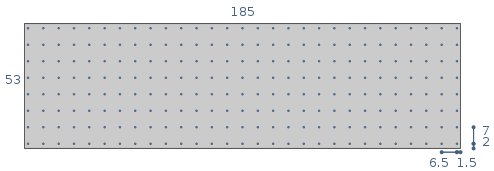
\includegraphics[width=.9\textwidth]{./figs/mh_dist.png}
\caption{Metal Halide luminaires distributed along the facility ceiling.}
\label{fig:mh_dist}
\end{figure}

\section{Calculus of Economy}

\subsection{Energy Consumption}
To calculate the energy consumption, the following data are needed:
\begin{itemize}
\item Number of luminaires: $232$
\item Energy cost: $0.093$\$
\item Electric demand cost: $11.00$\$
\item Number of hours per year: $16 \times 365.25 = 5,844$
\item Luminaire power: $458 W$
\end{itemize}
The numbers of hours per year assumes the leap year, so, the multiplier is $365.25$. The energy consumption results are showed as follow:
\begin{itemize}
\item Total power ($kW$): $232 \times 458 = 106,256 W = 106.256 kW$
\item Total electric demand cost per year: $11 \times 12 \times 106.256 = 14,025.79$\$
\item Total electric consumption cost per year: $5,844 \times 0.093 \times 106.256 = 57,749.29$\$
\item Total energy cost: $71,775.08$\$
\end{itemize}

\subsection{Average of Replaced Lamps per Year}
In order to calculate the average of lamps replaced per year, the following data are needed:
\begin{itemize}
\item Number of luminaires: $232$
\item Number of hours per year: $5,844$
\item Lamp lifetime hours at $80\%$ of survival: $14,000$
\end{itemize}

The Equation~\ref{eq:mh_relamp_average} shows the replaced lamps calculus.

\begin{equation}
\begin{split}
 & \text{Individual replaced lamps} \\
M_{individual} & = 20\% \times 232 \times \frac{5,844}{14,000} \\
 & = 19.37 \\
 & \approx 20
\end{split}
\begin{split}
 & \text{Collective replaced lamps} \\
M_{collective} & = 232 \times \frac {5,844}{14,000} \\
 & = 96.84 \\i
 & \approx 97
\end{split}
\label{eq:mh_relamp_average}
\end{equation}
Taking into account the worst case scenario, the calculation for this average is ceiling rounded. Thus, the average of replaced lamps per year is $117$.

\subsection{Relamping Workforce Cost per Year}
In order to calculate the cost for the relamping workforce per year, the following data are needed:
\begin{itemize}
\item Average of individual lamps replaced per year: $20$
\item Individual relamping cost: $87.00$\$
\item Average of collective luminaires replaced per year: $97$
\item Collective relamping cost: $9.00$\$
\end{itemize}

The average cost per year for the collective relamping is $873.00$\$ and for the individual relamping is $1,740,00$\$, so the total is $2.613,00$\$

